% Gemini theme
% https://github.com/anishathalye/gemini

\documentclass[final]{beamer}

% ====================
% Packages
% ====================

\usepackage[T1]{fontenc}
\usepackage{lmodern}
\usepackage[size=custom,width=100,height=70,scale=0.8]{beamerposter}
\usetheme{gemini}
\usecolortheme{eurecom}
\usepackage{graphicx}
\usepackage{epstopdf}  % Include the epstopdf package
\usepackage{booktabs}
\usepackage{tikz}
\usepackage{pgfplots}
\pgfplotsset{compat=1.14}
\usepackage{anyfontsize}
\usepackage{lipsum}
\usepackage{multicol}
\usepackage{comment} % Required for the comment environment
\usepackage{subcaption} % for subfigures
\usepackage{tabularx}
% ====================
% Lengths
% ====================

% If you have N columns, choose \sepwidth and \colwidth such that
% (N+1)*\sepwidth + N*\colwidth = \paperwidth
\newlength{\sepwidth}
\newlength{\colwidth}
\setlength{\sepwidth}{0.025\paperwidth}
\setlength{\colwidth}{0.3\paperwidth}

\renewcommand{\familydefault}{\sfdefault}

% ====================
% Title
% ====================

\title{\textsf{RF Oscillator and Wireless Transmitter}}
\author{ \textsf{ \textbf{Project Number:} 2896 \\
        \textbf{Names:} Mazz Shaikh \and Nir Finch Cohen\\ 
        \textbf{Advisor:} Edoh Shaulov
        }
    }

% ====================
% Header and Footer Colors
% ====================

% Set header and footer background color to white
\setbeamercolor{headline}{bg=white}
\setbeamercolor{footline}{bg=white}

% ====================
% Logo (optional)
% ====================

% Include Eurecom logo on the right side of the header
\logoleft{
\includegraphics[height=7cm]{./logos/TAU_new.jpeg}}
% Include Lab logo on the left side of the header
%\logoleft{
\includegraphics[height=7cm]{./logos/s3logo.png}}

% ====================
% Block Title Color
% ====================

% Set block title background color to white and text color to black
\setbeamercolor{block title}{fg=black}

% ====================

% Custom Command for Styled Section Titles
\newcommand{\mysection}[1]{%
    \par\vspace{0.5\baselineskip} % Adjust the space before the title
    \begin{center}
        {\usebeamerfont{section title}\textbf{\large\bfseries #1}\par} % Adjust the font size and weight (\large\bfseries)
    \end{center}
    \vspace{0.5\baselineskip} % Adjust the space after the title
}


% Explicitly set the title font to the default LaTeX font
\makeatletter
\setbeamertemplate{title page}{
    \vbox{}
    \vfill
    \begin{centering}
        {\usebeamerfont{title}\usebeamercolor[fg]{title}\rmfamily\inserttitle\par}
        \vskip0.5em
        {\usebeamerfont{subtitle}\usebeamercolor[fg]{subtitle}\insertsubtitle\par}
        \vskip1em
        {\usebeamerfont{author}\insertauthor\par}
        \vskip1em
        {\usebeamerfont{institute}\insertinstitute\par}
        \vskip1em
        {\usebeamerfont{date}\insertdate\par}
    \end{centering}
    \vfill
}

\makeatother

% Body
\begin{document}

\begin{frame}[t]

\begin{columns}[t]
\begin{column}{\colwidth}
\mysection{Introduction}
\section{Introduction}



\mysection{Motivation}

\begin{comment}
Our project set out to design, implement and fabricate an RF Oscillator, matching network and microstrip antenna on a PCB operating between 3.4 and 3.6GHz. We were centrally interested in understanding and implementing several of the main hardware building blocks found in communication systems.

\begin{enumerate}
\item Develop and validate a detailed Spice model for the selected transistor.
\item Design an oscillator circuit capable of generating the required frequency and analyze its stability, frequency accuracy, and harmonic content.
\item Design a matching network to achieve a \(50[\Omega]\) impedance match for the antenna and validate it through S-parameters analysis.
\item Develop and simulate the antenna system to be integrated into the transmitter, demonstrating efficiency and radiation patterns.
\item Fabricate the PCB according to the finalized layout, conduct comprehensive system testing, and validate performance metrics such as signal strength and reliability.
\end{enumerate}
\end{comment}

\begin{itemize}
    \item \textbf{Scientific Challenge}: Addressing the need for precise and stable oscillations at the 3.5 GHz frequency, crucial for modern wireless communication systems, including 5G networks and satellite communication.
    \item \textbf{Matching}: The design employs matching network to feed the load(Antenna) rather than a buffer, leading to space optimization.
    \item \textbf{Customization Requirement}: Overcoming the limitations of off-the-shelf oscillators that may not coincide with the characteristics of the antenna. Building both in parallel increases efficiency of design by ensuring the operating frequency stays in pass-band of antenna. 
    \item \textbf{System Reliability}: Designing a bespoke oscillator that ensures frequency stability, phase noise reduction, and power efficiency for a more reliable communication system.
    \item \textbf{Cost Efficiency}: Streamlining the design and manufacturing process to reduce production costs while maintaining high performance and reliability.
\end{itemize}

\mysection{Implementation}
\begin{figure}[h]
    \centering
    \begin{subfigure}[t]{0.64\textwidth}
        \centering
        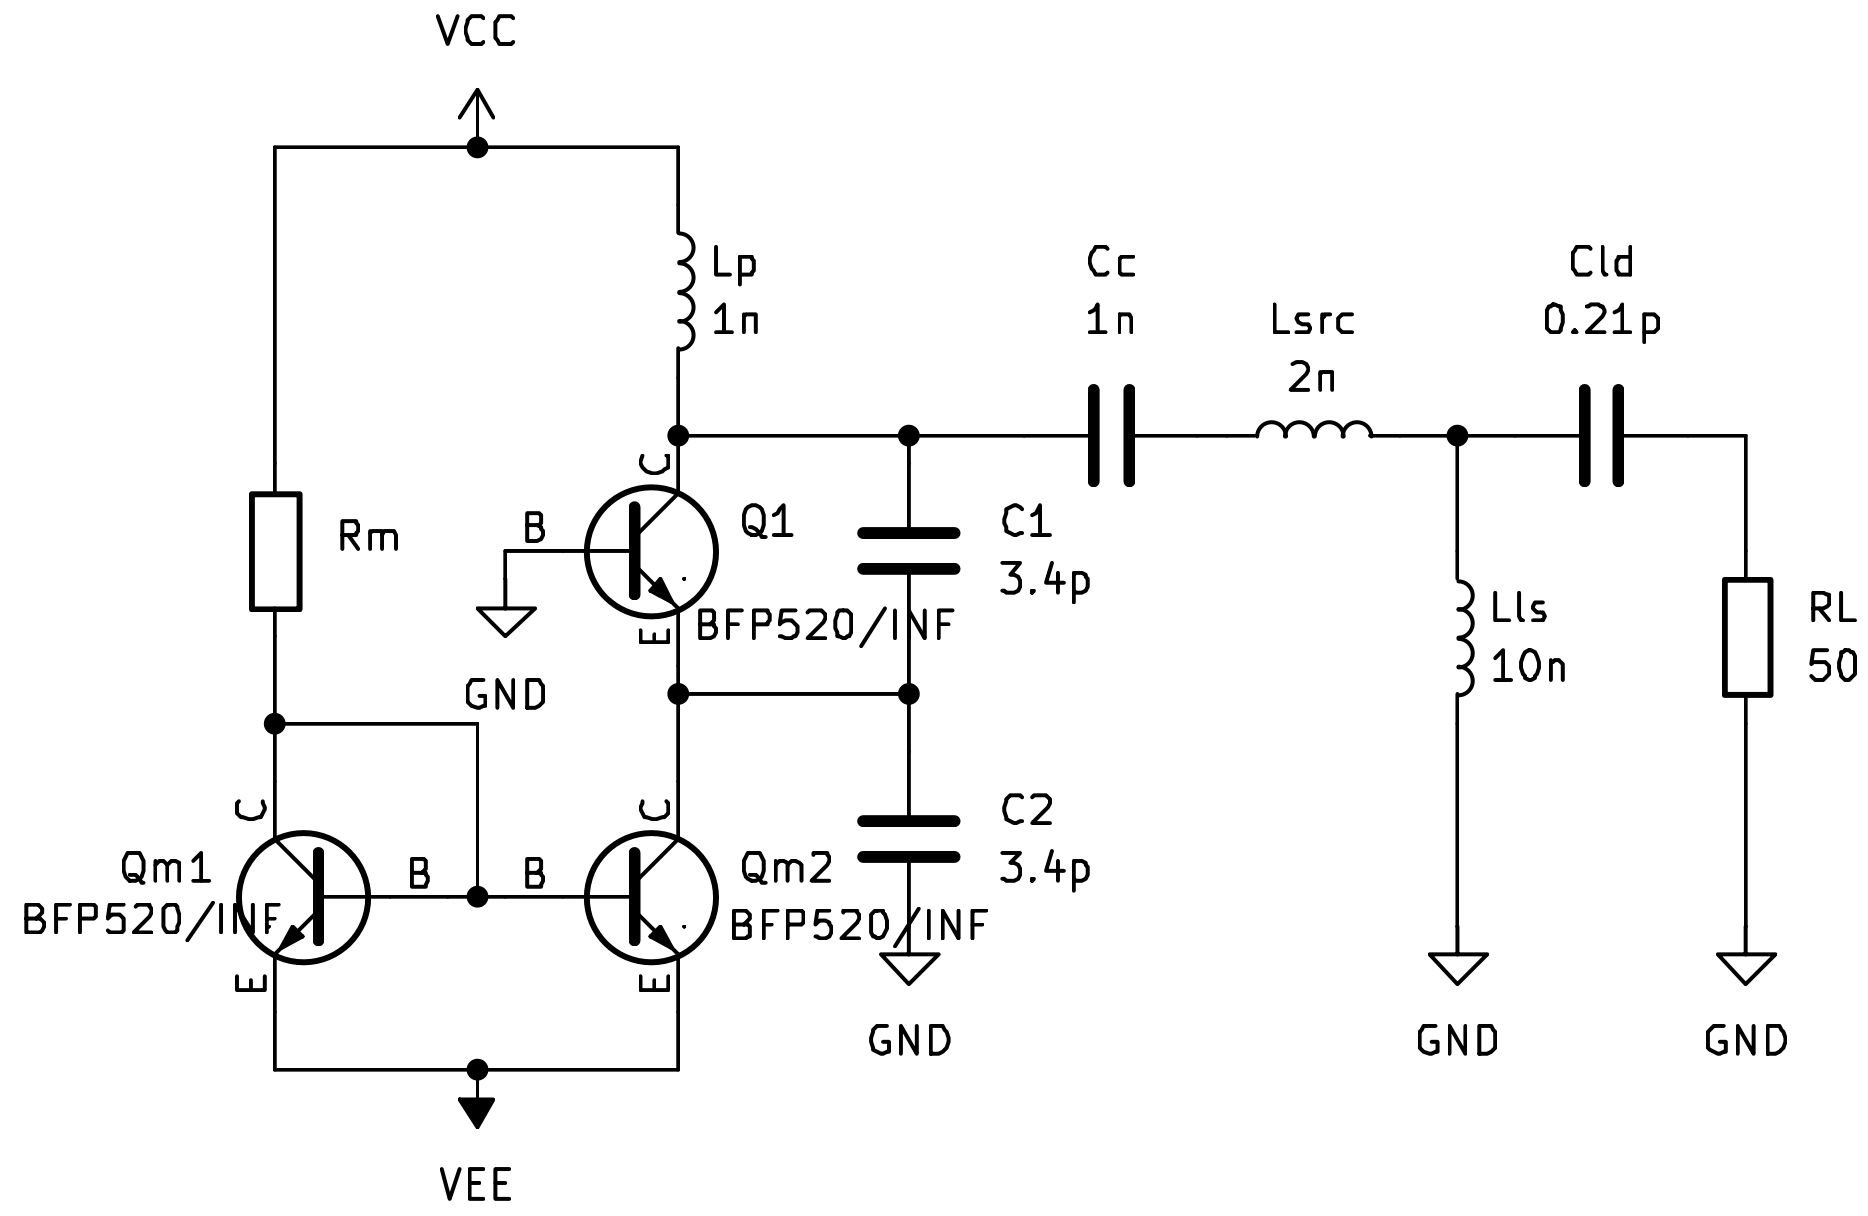
\includegraphics[width=\linewidth]{images/osc/osc_circuit.png}
        \caption{Oscillator+Matching Network Topology}
        \label{fig:osc_and_match}
    \end{subfigure}
    \hfill
    \begin{subfigure}[t]{0.35\textwidth}
        \centering
        \begin{tikzpicture}
            \definecolor{mycolor}{RGB}{200,200,200}
            % Draw a grey rectangle without borders
            \fill[mycolor] (0,0) rectangle (9,6.5);
            \fill[mycolor] (1, -1) rectangle (8, -0.5);
            \fill[mycolor] (4, -4.5) rectangle (5, -1);
            \fill (4.5, -1) circle (0.15);
            \fill[red] (4.5, -4.5) circle (0.15);
        \end{tikzpicture}
        \caption{Wideband Patch Antenna}
        \label{fig:patch-antenna}
    \end{subfigure}
    \caption{Design and Topology of primary components}
    \label{fig:combined}
\end{figure}

% ================================================ OSC =====================================

\textbf{Oscillator:}
The Colpitts oscillator topology is ideal for a\(3.5[GHz]\) oscillator due to its excellent frequency stability, making it suitable for precise frequency control in communication systems. Its easy tuning capability allows for straightforward frequency adjustments by changing capacitors and inductors. Additionally, Colpitts oscillators typically exhibit low phase noise, crucial for maintaining signal integrity and reducing interference in RF applications. The topology’s simplicity and cost-effectiveness further enhance its practicality, making it a preferred choice for stable and efficient\(3.5[GHz]\) oscillator designs. To ensure reliable functioning of the oscillator, startup conditions obtained using small-signal analysis were withheld~\cite{Johnson1986ACO}. The SSM gave us
\[\frac{v_{out}}{i_{in}} = \frac{r_\pi L_p R_L(s^2C + sg_m)}{r_\pi C^2L_p R_L s^3  +(- r\pi C L_p R_L g_m + 2r_\pi CL_p + CL_pR_L)s^2 + (2r_\pi CR_L + L_p)s + R_L}\]
We attained conditions: \(\displaystyle \omega_0 \approx \sqrt{\frac{1}{\displaystyle L\frac{C_1 C_2}{C_1+C_2}}}\)\footnote{Assuming \(r_\pi (C_1+C_2)R_L >> L_p\)} and \(\displaystyle R_L (g_m) - \frac{R_L}{(r_\pi)} - 2 > 0\)

\begin{comment}
After deciding on the Colpitts topology, startup conditions were derived from the following small signal-based equation: \(\displaystyle i_{in} = -\frac{v_{\pi}}{r_{\pi}} - sC(v_{out} + 2v_{\pi})\) and \(\displaystyle 0 = g_mv_{\pi} + sC(v_{out} + v_{\pi}) + \frac{v_{out}}{sL_p} + \frac{v_{out}}{R_L}\).

We attained the approximation for operating frequency and startup condition: \(\displaystyle \omega_0 \approx \sqrt{\frac{1}{L\frac{C_1 C_2}{C_1+C_2}}}\) and \(\displaystyle R_L g_m - \frac{R_L}{r_\pi} - 2 > 0\).\par
\end{comment}



\end{column}

\begin{column}{\colwidth}

% ================================================ MATCHING =====================================
\textbf{Matching:}
A T-Matching Network was used since it offers more control over the Q factor compared to L-match but with a trade-off of slightly more complex design~\cite{Pozar:882338}. The values of \(L, C\) were approximated to available component values.\par

% ================================================ ANTENA =====================================
\textbf{Antenna:}
Regular microstrip patch antennas generally have a narrow bandwidth. This makes them less suitable for wideband applications. To handle fabrication variations in the oscillating frequency, a different topology consisting of coupled resonators was used~\cite{7592896}. This improves BW by providing two controllable resonances and supression of extra harmonics in the vicinity.\par


% ======================== PCB ======================

\mysection{Results}
\textbf{Oscillator System:}(\ref{fig:osc_and_match}) The Spectre simulation of the oscillator system gives (\ref{fig:osc_trans}) as it's transient waveform on \(R_L\) with frequencies shown in Figure (\ref{fig:osc_spec}). 

A maximum attainable efficiency of \(19.8\%\)(based on \(V_{cc}, V_{ee}\)) was measured.
\begin{comment}
\begin{figure}[htbp]
    \centering
    \begin{subfigure}[b]{0.49\textwidth}
        \centering
        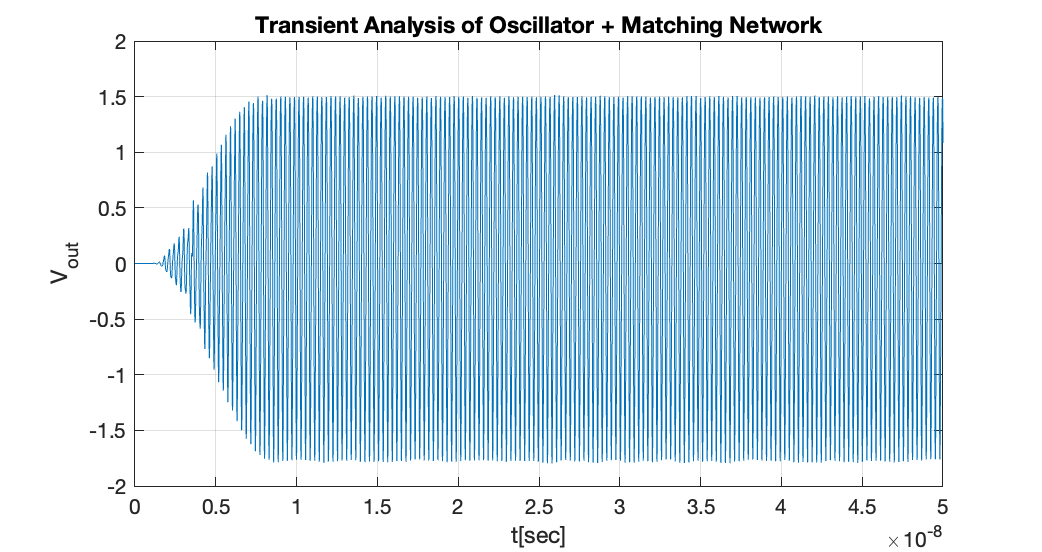
\includegraphics[width=\textwidth]{images/osc/VCO_trans.png}
        \caption{Transient Analysis of Oscillator}
        \label{fig:osc_trans}
    \end{subfigure}
    \hfill % horizontal space between subfigures
    \begin{subfigure}[b]{0.49\textwidth}
        \centering
        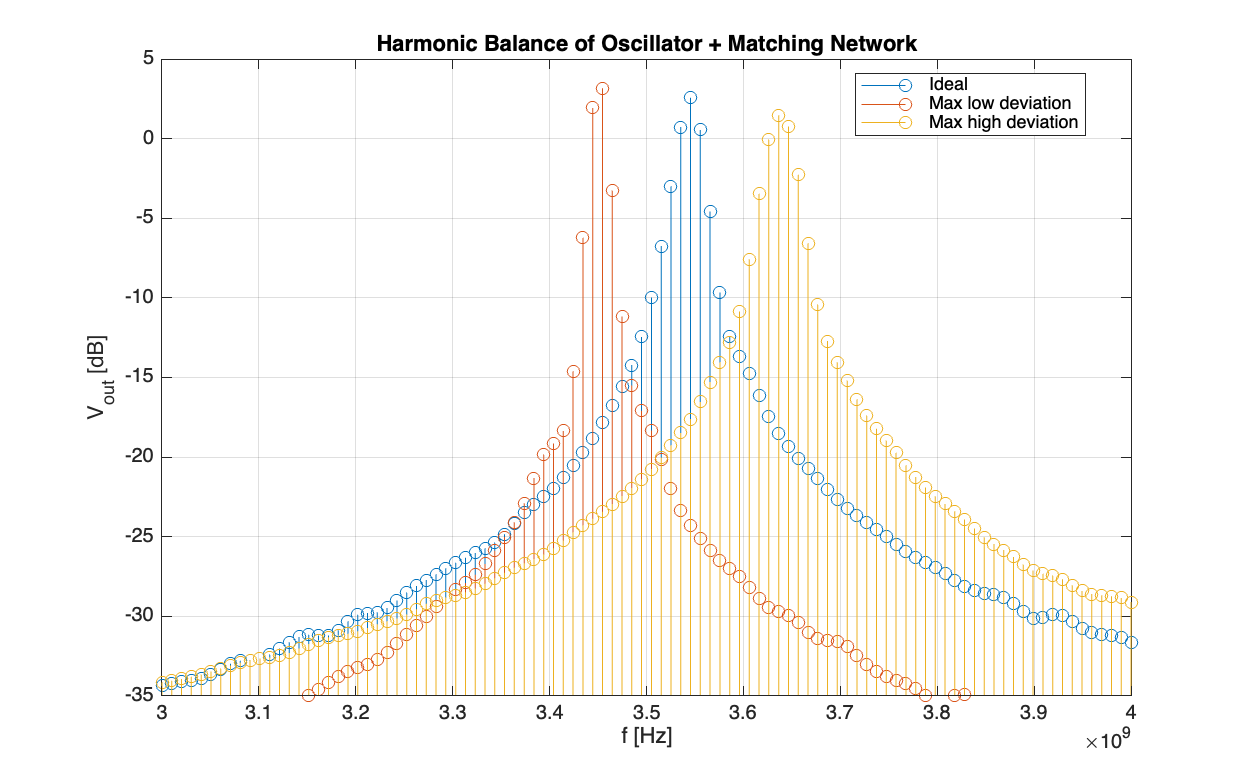
\includegraphics[width=\textwidth]{images/osc/VCO_spec_smoothed_with_peak_values.png}
        \caption{Spectral Analysis of Oscillator}
        \label{fig:osc_spec}
    \end{subfigure}
    \caption{Oscillator Outputs}
    \label{fig:osc}
\end{figure}
\end{comment}

\begin{figure}
    \centering
    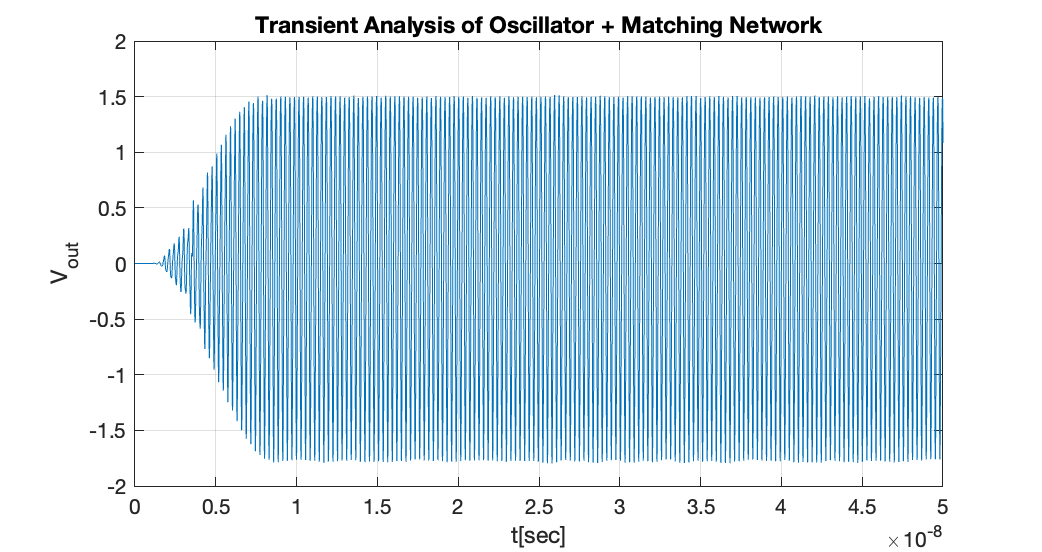
\includegraphics[width=0.95\textwidth]{images/osc/VCO_trans.png}
    \caption{Transient Analysis of Oscillator}
    \label{fig:osc_trans}
\end{figure}

Possible deviations due to non-idealities in the components need to be computed to ensure reliable functioning in the worst-case scenario. In accordance with manufacturer specification of the components used, the operating frequency was found to be in the range \(3.454[GHz]\to 3.636[GHz]\).\par

\begin{figure}
    \centering
    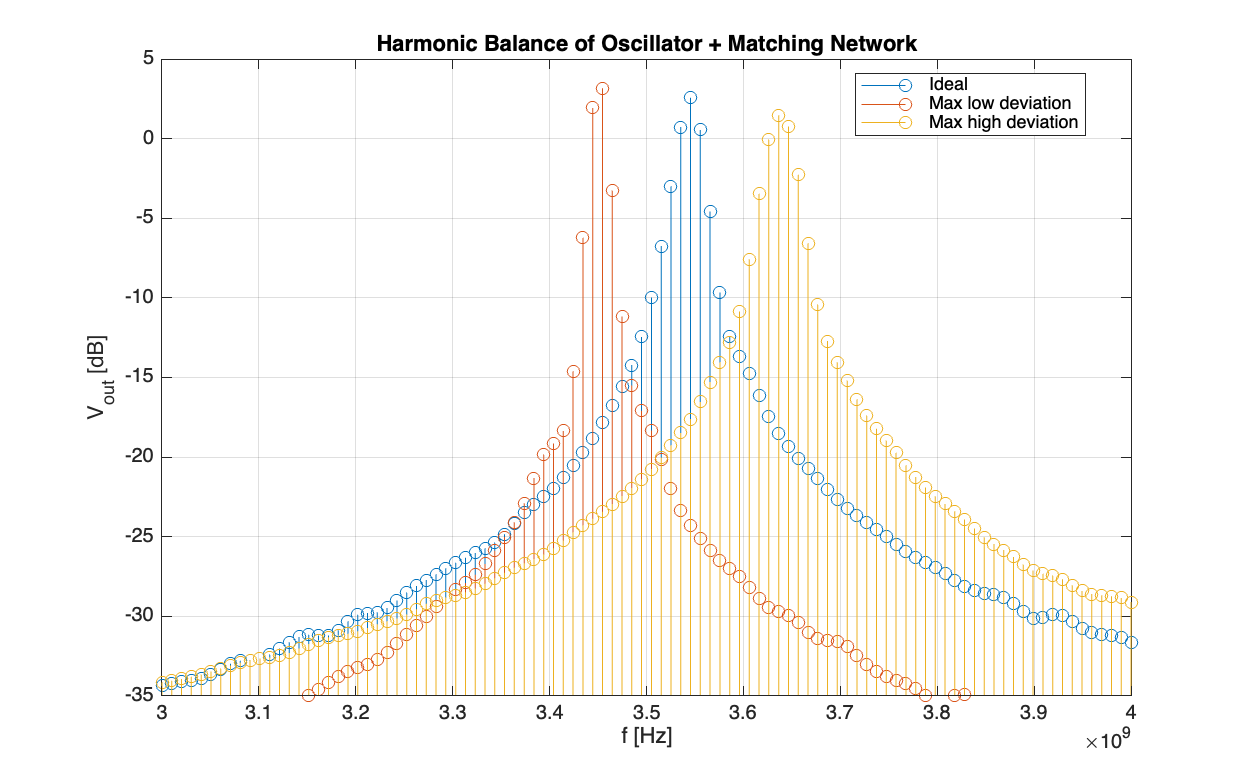
\includegraphics[width=0.9\textwidth]{images/osc/VCO_spec_smoothed_with_peak_values.png}
    \caption{Spectral Analysis of Oscillator}
    \label{fig:osc_spec}
\end{figure}

\begin{comment}
\begin{figure}
    \centering
    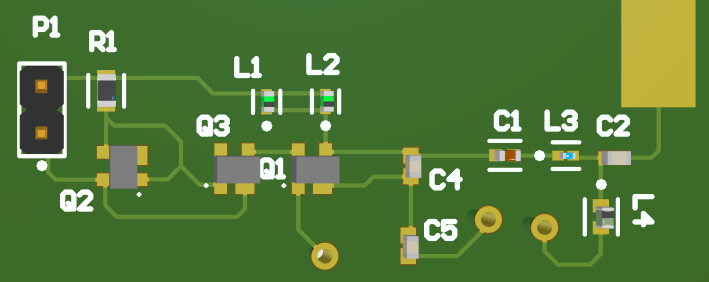
\includegraphics[width=0.85\textwidth]{images/layout/board3.png}
    \caption{3D Layout without Antenna}
    \label{fig:3DLayout}
\end{figure}
\end{comment}


\textbf{Antenna:}(\ref{fig:patch-antenna})
Scattering parameters were simulated for wide band micro-strip antenna as seen in Figure (\ref{fig:antenna_s}). The bandwidth was computed to be \(3.441[GHz]\to 3.642[Ghz]\), ensuring the deviations in oscillation frequency stay in \(S_{11}<-10[dB]\).

\begin{table}[H]
\centering
\caption{Far-Field Characteristics of Wideband Microstrip Antenna}
\label{table:antenna_characteristics}
\begin{tabularx}{0.7\linewidth}{|X|X|}
\hline
\textbf{Parameter} & \textbf{Value} \\
\hline
Main Lobe Magnitude & 6.22 dBi \\
Main Lobe Direction & 0.0 deg \\
Angular Width at 3 dB & 79.9 deg \\
Side Lobe Level & -15.6 dBi \\
\hline
\end{tabularx}
\end{table}

\end{column}

\begin{column}{\colwidth}
\begin{figure}[htbp]
    \centering
    \begin{subfigure}[b]{0.49\textwidth}
        \centering
        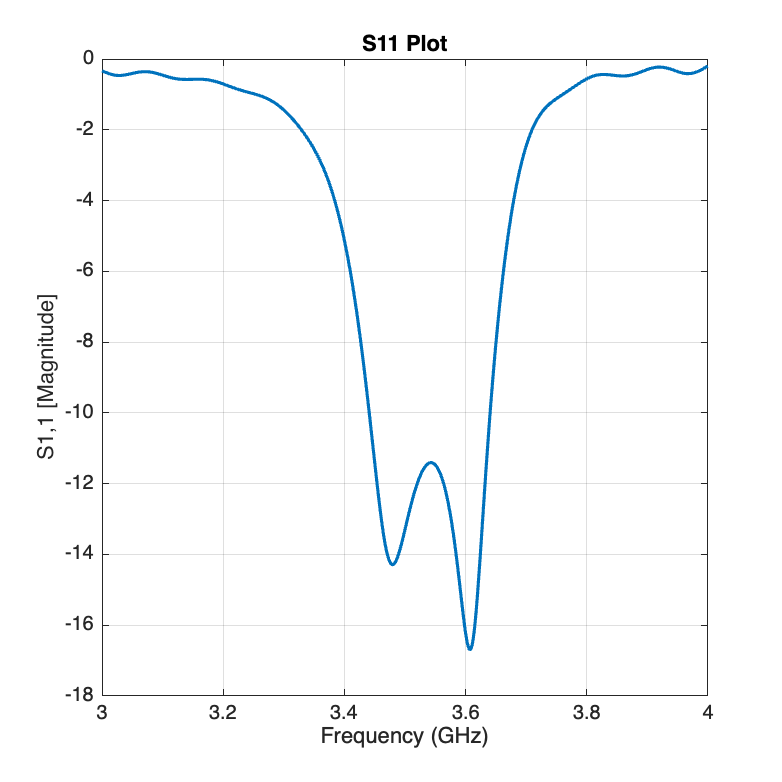
\includegraphics[width=\textwidth]{images/antenna/S11.png}
        \caption{S-parameters of Antenna}
        \label{fig:antenna_s}
    \end{subfigure}
    \hfill % horizontal space between subfigures
    \begin{subfigure}[b]{0.49\textwidth}
        \centering
        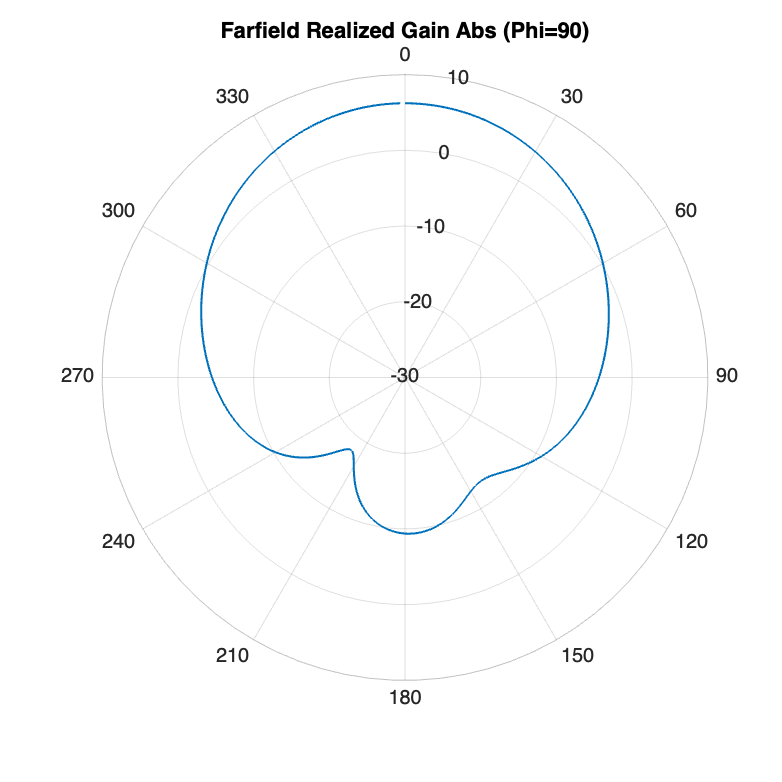
\includegraphics[width=\textwidth]{images/antenna/FF_p.png}
        \caption{Far Field Distribution}
        \label{fig:antenna_ff}
    \end{subfigure}
    \caption{Antenna Outputs}
    \label{fig:ant}
\end{figure}


\begin{comment}
\begin{figure}
    \centering
    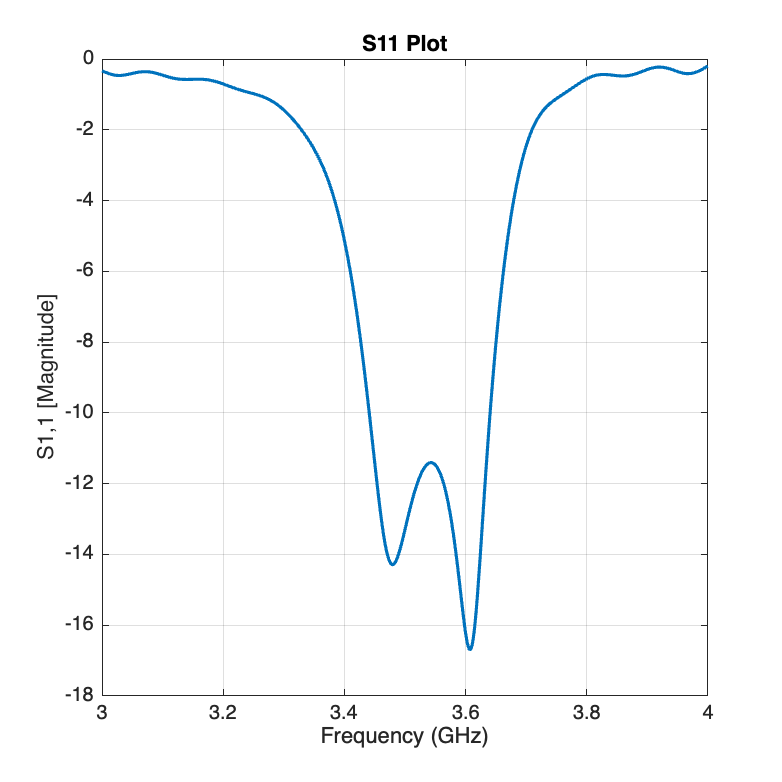
\includegraphics[width=0.8\textwidth]{images/antenna/S11.png}
    \caption{S-parameters of Antenna}
    \label{fig:antenna_s}
\end{figure}

\begin{figure}
    \centering
    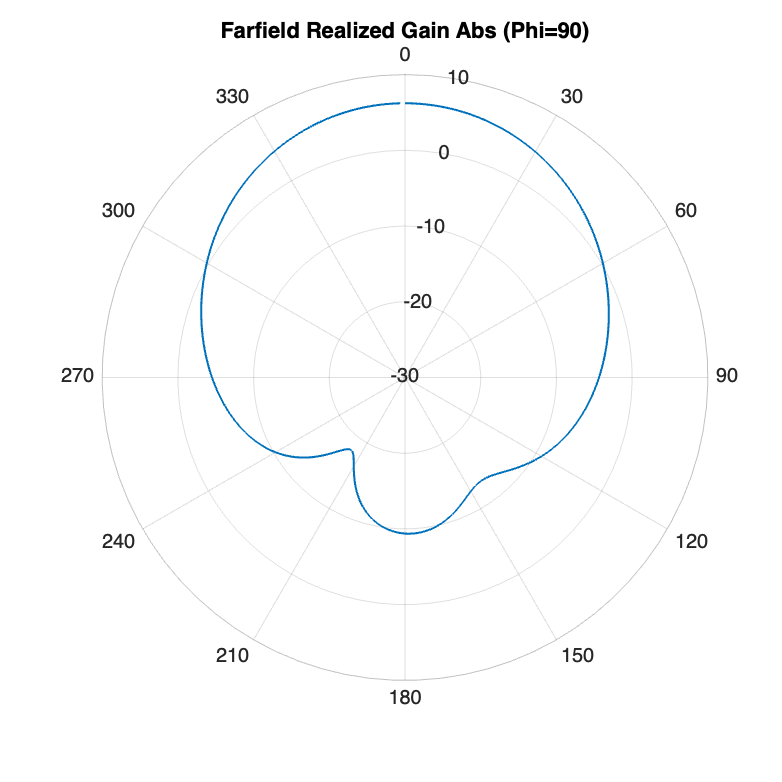
\includegraphics[width=0.8\textwidth]{images/antenna/FF_p.png}
    \caption{Far Field Distribution}
    \label{fig:antenna_ff}
\end{figure}
\end{comment}

The far-field characteristics of the microstrip patch antenna seen in Figure (\ref{fig:antenna_ff}) and Table (\ref{table:antenna_characteristics}), having a main lobe magnitude of \(6.22 [dBi]\), a side lobe level of \(-15.6 [dBi]\), and an angular width of \(79.9 \deg\) at \(3 [dB]\), demonstrate typical performance metrics for such antennas, indicating efficient radiation and low interference from side lobes.


\textbf{Fabrication:}
The circuit, matching network and antenna were layed out in Altium and sent for fabrication. CST-provided specs were used when deciding the board dimensions, so as to preclude fringing affects. The final layout of just the circuit section is seen in Figure (\(\ref{fig:board}\)).
\begin{figure}
    \centering
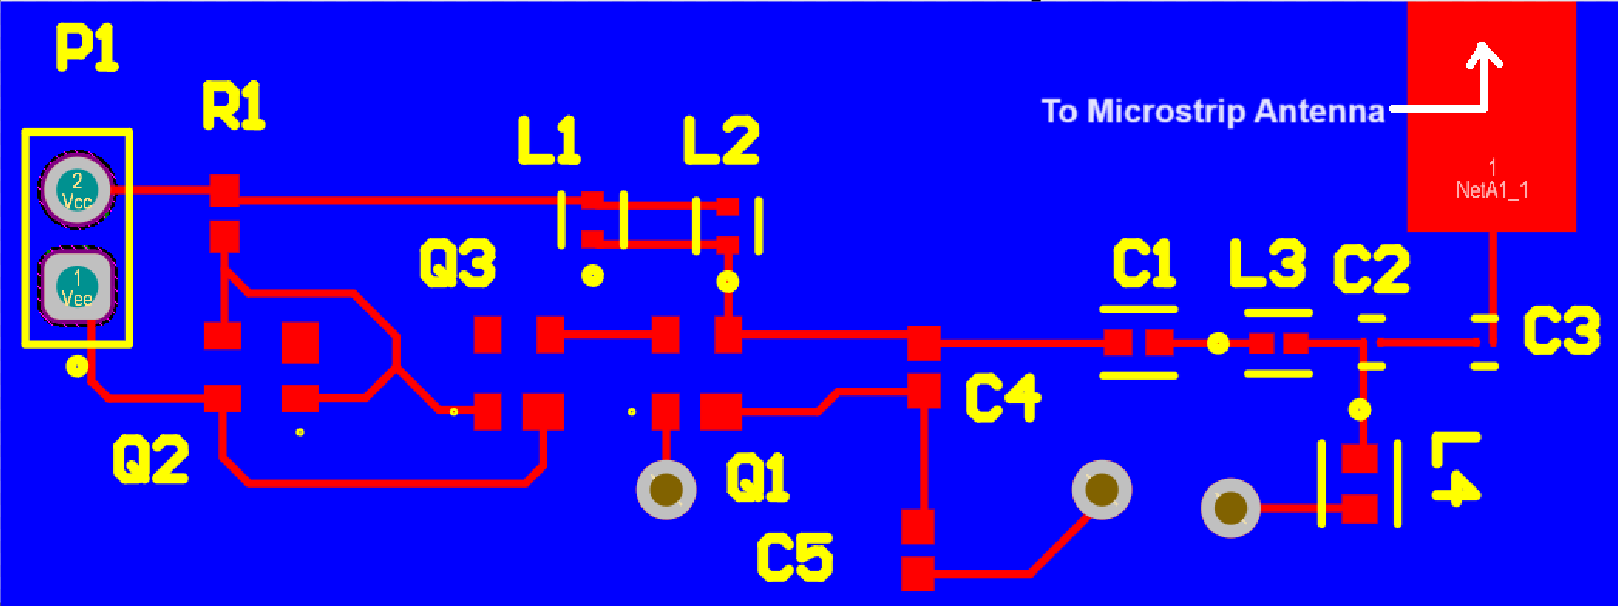
\includegraphics[width=0.9\textwidth]{images/layout/board.png}
    \caption{Altium Board Layout}
    \label{fig:board}
\end{figure}
The circuit was sent to JLC-PCB for fabrication and will be spectrally tested in the RFIC lab. The spectrum of the transmitted output should be a single spike in the frequency domain at \(3.5[GHz]\).
\mysection{Conclusion}
Simulations show the functioning of all of the oscillator, matching network and microstrip antenna in producing and transmitting the \(3.5[GHz]\) signal. This has been verified by transient and spectral analysis of the output of the circuit itself and by the simulated pass-band of the microstrip antenna. According to simulations, we were able to obtain good efficiency in oscillator and large enough bandwidth in the antenna to cover the cases of maximum deviation from ideal oscillating frequency, ensuring reliable performance in edge cases as well. \par


Upon delivery of the PCB, the output of the antenna will be detected and spectrally analysed in the RFIC lab. The key parts of this project exemplify three of the most significant building blocks of modern wireless communication systems.

\mysection{References}


    \nocite{*}
    \footnotesize{\bibliographystyle{plain}\bibliography{poster}}

\end{column}
\end{columns}

\end{frame}

\end{document}
